\documentclass[tikz,border=8pt]{standalone}
% Shared look for every TikZ diagram. Load with % Shared look for every TikZ diagram. Load with % Shared look for every TikZ diagram. Load with \input{../../tools/tikz-style.tex}
\usepackage[T1]{fontenc}
\usepackage{lmodern}
\renewcommand{\sfdefault}{lmr}  % diagrams use the same serif as the text
\usetikzlibrary{arrows.meta, positioning, shapes.geometric, calc, fit, backgrounds}
\definecolor{cblue}{HTML}{4C78A8}
\definecolor{corange}{HTML}{F58518}
\definecolor{cgreen}{HTML}{54A24B}
\definecolor{cred}{HTML}{E45756}
\definecolor{cpurple}{HTML}{B279A2}
\definecolor{cgrey}{HTML}{6B6B6B}
\tikzset{
  every picture/.style={font=\sffamily, line width=1.2pt},
  box/.style={draw=#1, fill=#1!12, rounded corners=4pt, align=center, inner sep=7pt, minimum height=1.1cm},
  box/.default=cgrey,
  arrow/.style={-{Stealth[length=3mm]}, draw=cgrey, line width=1.4pt},
  title/.style={font=\sffamily\bfseries\Large},
  note/.style={font=\sffamily\small, text=cgrey, align=center},
}
\AtBeginDocument{\hyphenpenalty=10000 \exhyphenpenalty=10000}

\usepackage[T1]{fontenc}
\usepackage{lmodern}
\renewcommand{\sfdefault}{lmr}  % diagrams use the same serif as the text
\usetikzlibrary{arrows.meta, positioning, shapes.geometric, calc, fit, backgrounds}
\definecolor{cblue}{HTML}{4C78A8}
\definecolor{corange}{HTML}{F58518}
\definecolor{cgreen}{HTML}{54A24B}
\definecolor{cred}{HTML}{E45756}
\definecolor{cpurple}{HTML}{B279A2}
\definecolor{cgrey}{HTML}{6B6B6B}
\tikzset{
  every picture/.style={font=\sffamily, line width=1.2pt},
  box/.style={draw=#1, fill=#1!12, rounded corners=4pt, align=center, inner sep=7pt, minimum height=1.1cm},
  box/.default=cgrey,
  arrow/.style={-{Stealth[length=3mm]}, draw=cgrey, line width=1.4pt},
  title/.style={font=\sffamily\bfseries\Large},
  note/.style={font=\sffamily\small, text=cgrey, align=center},
}
\AtBeginDocument{\hyphenpenalty=10000 \exhyphenpenalty=10000}

\usepackage[T1]{fontenc}
\usepackage{lmodern}
\renewcommand{\sfdefault}{lmr}  % diagrams use the same serif as the text
\usetikzlibrary{arrows.meta, positioning, shapes.geometric, calc, fit, backgrounds}
\definecolor{cblue}{HTML}{4C78A8}
\definecolor{corange}{HTML}{F58518}
\definecolor{cgreen}{HTML}{54A24B}
\definecolor{cred}{HTML}{E45756}
\definecolor{cpurple}{HTML}{B279A2}
\definecolor{cgrey}{HTML}{6B6B6B}
\tikzset{
  every picture/.style={font=\sffamily, line width=1.2pt},
  box/.style={draw=#1, fill=#1!12, rounded corners=4pt, align=center, inner sep=7pt, minimum height=1.1cm},
  box/.default=cgrey,
  arrow/.style={-{Stealth[length=3mm]}, draw=cgrey, line width=1.4pt},
  title/.style={font=\sffamily\bfseries\Large},
  note/.style={font=\sffamily\small, text=cgrey, align=center},
}
\AtBeginDocument{\hyphenpenalty=10000 \exhyphenpenalty=10000}

\begin{document}
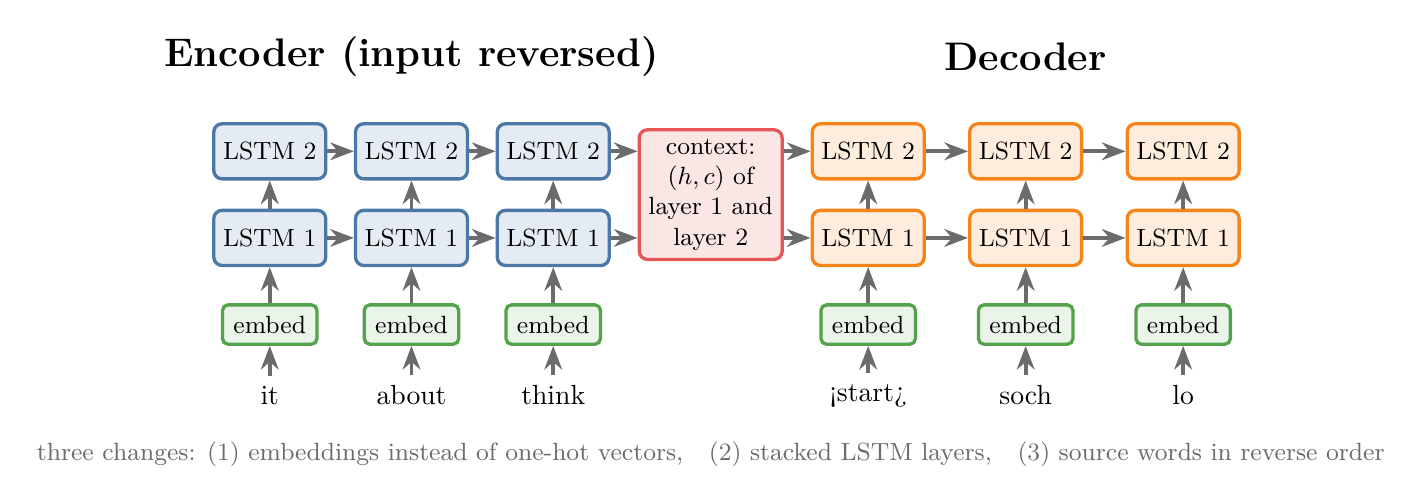
\begin{tikzpicture}[cell/.style={draw=#1, fill=#1!15, minimum width=1.2cm, minimum height=0.7cm, rounded corners=3pt, font=\sffamily\small},
  emb/.style={draw=cgreen, fill=cgreen!12, minimum width=1.2cm, minimum height=0.5cm, rounded corners=2pt, font=\sffamily\small},
  word/.style={font=\sffamily}]
  \node[title] at (2.8, 4.3) {Encoder (input reversed)};
  \node[title] at (10.6, 4.3) {Decoder};
  % encoder: words reversed
  \foreach \w [count=\i] in {it, about, think} {
    \node[emb] (ee\i) at (1.8*\i - 0.8, 0.9) {embed};
    \node[cell=cblue] (a\i) at (1.8*\i - 0.8, 2.0) {LSTM 1};
    \node[cell=cblue] (b\i) at (1.8*\i - 0.8, 3.1) {LSTM 2};
    \node[word] (x\i) at (1.8*\i - 0.8, 0.0) {\w};
    \draw[arrow] (x\i) -- (ee\i); \draw[arrow] (ee\i) -- (a\i); \draw[arrow] (a\i) -- (b\i);
  }
  \foreach \i/\j in {1/2, 2/3} { \draw[arrow] (a\i) -- (a\j); \draw[arrow] (b\i) -- (b\j); }
  % context: one (h, c) pair per layer
  \node[draw=cred, fill=cred!15, rounded corners=3pt, font=\sffamily\small, align=center] (c) at (6.6, 2.55) {context:\\$(h, c)$ of\\layer 1 and\\layer 2};
  \draw[arrow] (a3.east) -- (c.west |- a3.east);
  \draw[arrow] (b3.east) -- (c.west |- b3.east);
  % decoder
  \foreach \w [count=\i] in {{<start>}, soch, lo} {
    \node[emb] (ed\i) at (6.6 + 2.0*\i, 0.9) {embed};
    \node[cell=corange] (p\i) at (6.6 + 2.0*\i, 2.0) {LSTM 1};
    \node[cell=corange] (q\i) at (6.6 + 2.0*\i, 3.1) {LSTM 2};
    \node[word] (y\i) at (6.6 + 2.0*\i, 0.0) {\w};
    \draw[arrow] (y\i) -- (ed\i); \draw[arrow] (ed\i) -- (p\i); \draw[arrow] (p\i) -- (q\i);
  }
  \foreach \i/\j in {1/2, 2/3} { \draw[arrow] (p\i) -- (p\j); \draw[arrow] (q\i) -- (q\j); }
  \draw[arrow] (c.east |- p1.west) -- (p1.west);
  \draw[arrow] (c.east |- q1.west) -- (q1.west);
  \node[note] at (6.6, -0.75) {three changes: (1) embeddings instead of one-hot vectors,\quad (2) stacked LSTM layers,\quad (3) source words in reverse order};
\end{tikzpicture}
\end{document}
